\documentclass[11pt,reqno]{amsart}

\usepackage[margin=1in]{geometry}
\usepackage{amsmath,amssymb,amsthm,mathtools}
\usepackage{booktabs,array,multirow}
\usepackage{graphicx}
\usepackage{microtype}
\usepackage[dvipsnames]{xcolor}
\usepackage[colorlinks=true,linkcolor=NavyBlue,citecolor=ForestGreen,urlcolor=RoyalBlue]{hyperref}
\usepackage[capitalise,noabbrev]{cleveref}
\raggedbottom

\newtheorem{theorem}{Theorem}[section]
\newtheorem{lemma}[theorem]{Lemma}
\newtheorem{proposition}[theorem]{Proposition}
\newtheorem{corollary}[theorem]{Corollary}
\theoremstyle{definition}
\newtheorem{definition}[theorem]{Definition}
\newtheorem{remark}[theorem]{Remark}
\newtheorem{openproblem}[theorem]{Open Problem}

\newcommand{\F}{\mathbb{F}}
\newcommand{\Q}{\mathbb{Q}}
\newcommand{\Z}{\mathbb{Z}}
\newcommand{\N}{\mathbb{N}}
\newcommand{\R}{\mathbb{R}}
\newcommand{\RP}{\mathrm{RP}}
\newcommand{\pass}{\mathrm{pass}}
\newcommand{\MC}{\mathrm{MC}_\wedge}

\title[Positive-Characteristic Dichotomy and Three-Register Catalytic Exponents]{%
  Positive-Characteristic Dichotomy and Optimal Three-Register Exponents\\
  in Passive Catalytic Register Programs}

\author{Alexander S. Donahue}
\address{Independent Researcher, Spokane, WA, USA}
\email{0\_0@0thernes.art}
\thanks{ORCID: \href{https://orcid.org/0009-0006-8168-9648}{0009-0006-8168-9648}.
Code and Lean~4.35.0 proofs are dual-licensed under Apache-2.0; prose and figures under CC-BY-4.0.
This work has not undergone external peer review; all formal proofs are independently certified by six Lean~4.35.0 verification kernels across five independent implementations.}

\date{November 23, 2026}

\subjclass[2020]{68Q06, 68Q15, 11T06, 12E20}
\keywords{Catalytic computing, register programs, finite fields, Lucas's theorem, powering algorithms, streaming algorithms, matrix powering, Lean~4 formal verification}

\begin{document}

\begin{abstract}
We resolve two structural questions left open by Vinciguerra's operator analysis of passive-output catalytic register programs (\href{https://arxiv.org/abs/2609.18692}{\texttt{arXiv:2609.18692}}, September~2026) and connect them to bilinear catalytic algebra and Boolean multiplicative complexity.
\begin{enumerate}
  \item \emph{Exact positive-characteristic two-register dichotomy (Theorem~\ref{thm:T1}).}
  Over any prime field $\F_p$, every budget $t \ge 1$, and every polynomial $f(x) = \sum_{d \ge 0}\alpha_d x^d \in \F_p[x]$, we prove the unconditional equivalence
  \[
    f \in \RP_{\F_p}^{\pass}(2, t) \iff \forall\, d \ge 2 \text{ with } \alpha_d \neq 0,\;\; s_p(d) \le \min(p-1,\, t-1),
  \]
  where $s_p(d)$ denotes the sum of the base-$p$ digits of $d$.
  Consequently, the characteristic-$0$ lower bounds of~\cite[Theorems~3.2, 3.3, and~3.5]{Vinciguerra2026} collapse completely in every positive prime characteristic: $D_{2,\F_p}^{\pass}(2) = +\infty$ via the Frobenius monomials $x^{p^m}$ ($s_p(p^m)=1$), whereas every degree with $s_p(d) \ge p$ (such as $x^3$ over $\F_2$) is permanently uncomputable in two passive registers for \emph{all} $t \ge 1$.
  When $p > \deg f$, the criterion reduces to $t \ge \deg f + 1$, recovering Vinciguerra's Theorem~3.5.

  \item \emph{Strictly bilinear two-access Frobenius collapse (Theorem~\ref{thm:T2}).}
  Over any commutative ring of characteristic~$2$, we construct an explicit passive-output program using strictly bilinear basic instructions ($R_i \leftarrow R_i + R_j R_\ell$ with $j,\ell \neq i$) that cleanly computes $x^{2^k}$ in $k+1$ registers, $4k-2$ bilinear operations, and \emph{only two} input accesses for every $k \ge 1$.

  \item \emph{Strict improvement over Vinciguerra's three-register powering exponent (Theorem~\ref{thm:T3}).}
  Using explicit elementary shear loops with integer Pascal-row coefficients, we prove $x^7 \in \RP_K^{\pass}(3, 5)$ (for all $\operatorname{char}(K) \neq 2, 3$), $x^9 \in \RP_K^{\pass}(3, 6)$ ($\operatorname{char}(K) \notin \{2,3,5,17\}$), $x^{11} \in \RP_K^{\pass}(3, 7)$, and $x^{13} \in \RP_K^{\pass}(3, 8)$ over $\Q$ and all good prime fields.
  This improves the three-register composition exponent from Vinciguerra's $\log_5 4 \approx 0.86135$ down to the unique integer minimizer $\log_{13} 8 \approx 0.81071$ of $\log_{2t-3} t$, immediately tightening the asymptotic exponents for $4$-register powering (Corollary~4.3.1), catalytic streaming frequency moments (Corollary~5.1.1), and $3$-register matrix powering (Theorem~5.2) of~\cite{Vinciguerra2026}.

  \item \emph{Balanced zero-workspace bilinear multilinear product (Theorem~\ref{thm:T4}).}
  Over any commutative ring, we formalize a recursive zero-workspace commutator computing $x_0 \cdots x_{d-1}$ ($d = 2^k$) using $\log_2 d + 2$ registers and exactly $(7d^2 - 4)/3$ primitive operations.
\end{enumerate}
All twelve main theorem and corollary statements together with explicit non-trivial ($0 \neq 1$) non-vacuity witnesses are formalized with zero Mathlib dependencies across eleven Lean~4.35.0 \texttt{module} files, depend strictly on the standard axiom set $\{\texttt{propext}, \texttt{Classical.choice}, \texttt{Quot.sound}\}$, and pass six independent verification kernel runs across five implementations (\texttt{lean}, \texttt{leanchecker}, \texttt{leanchecker-paranoid}, \texttt{con-leche}, \texttt{con-ron}, and \texttt{nanoda\_bin}).
An accompanying CaDiCaL~2.1.2 SAT audit (cross-checked against an independent brute-force enumerator on $n = 2, 3$) contrasts these catalytic gains against the rigidity of nonlinear cancellation in Boolean XAG circuits~\cite{BoyarFind2018,Morse2026}.
\end{abstract}

\maketitle

\section{Introduction and Main Results}
\label{sec:intro}

Catalytic computation, introduced by Buhrman, Cleve, Kouck\'y, Loff, and Speelman~\cite{BCKLS2014}, augments a space-bounded machine with a large \emph{catalytic} tape initialized to an arbitrary unknown state $\tau$ that must be restored bit-for-bit upon halting.
Following the breakthroughs of Cook and Mertz~\cite{CookMertz2024} on tree evaluation and Williams~\cite{Williams2025} on time--space simulation, algebraic \emph{register programs}~\cite{CoppersmithGrossman1975,BenOrCleve1992,AFM2025} have emerged as the primary engine for designing clean catalytic algorithms with sharp resource trade-offs.

In September~2026, Vinciguerra~\cite{Vinciguerra2026} introduced a Lie-theoretic operator representation for \emph{passive-output} register programs over fields of characteristic~$0$, writing $\RP_K^{\pass}(r, t)$ for the univariate polynomials cleanly computable using $r$ registers and at most $t$ input accesses without ever reading the output register, and setting $D_{r,K}^{\pass}(t) = \sup\{\deg f : f \in \RP_K^{\pass}(r, t)\}$.
Vinciguerra established three foundational results over characteristic~$0$:
\begin{itemize}
  \item $D_{r,K}^{\pass}(1) = D_{r,K}^{\pass}(2) = 1$ and $D_{r,K}^{\pass}(3) = 2$ for every $r \ge 2$ (\cite[Theorems~3.2 and~3.3]{Vinciguerra2026});
  \item $D_{2,K}^{\pass}(t) = t - 1$ for every $t \ge 1$ (\cite[Theorem~3.5]{Vinciguerra2026});
  \item $x^{2r-1} \in \RP_K^{\pass}(r, 4)$ for every $r \ge 2$ and $\operatorname{char}(K) = 0$ or $> 2r-1$ (\cite[Theorem~2.3]{Vinciguerra2026}), which for $r = 3$ yields $x^5 \in \RP_K^{\pass}(3, 4)$ and recursive powering exponent $\log_5 4 \approx 0.861353$.
\end{itemize}

Vinciguerra's operator proofs rely essentially on the formal exponential $\exp(x D) = \sum_{n \ge 0} \frac{x^n}{n!} D^n$ and the Campbell--Baker--Hausdorff formula, leaving open two sharp structural questions:
\begin{enumerate}
  \item[(Q1)] \emph{Positive-characteristic behavior:} What is the exact computational power of $\RP_{\F_p}^{\pass}(r, t)$ over prime fields $\F_p$, where $n!$ ceases to be invertible at $n = p$ and the Frobenius identity $a^p = a$ acts on instruction shifts?
  \item[(Q2)] \emph{Beyond four input accesses ($t \ge 5$):} Does the $r = 3$ four-call base program $x^5 \in \RP_K^{\pass}(3, 4)$ achieve the optimal three-register powering exponent $\log_5 4$, or can $t \ge 5$ input accesses achieve a strictly smaller recursive exponent $\log_N t$?
\end{enumerate}

In this paper we answer both (Q1) (completely for $r = 2$, and for bilinear programs of arbitrary $r$ over characteristic~$2$) and (Q2) (strictly improving the $r = 3$ exponent from $0.861353$ to $0.810714$), unify them with an optimal balanced zero-workspace bilinear multilinear product, and contrast the power of nonlinear cancellation in catalytic programs with its apparent rigidity in Boolean XAG multiplicative complexity~\cite{BoyarFind2018,Morse2026}.

\subsection{Summary of Main Theorems}

Let $s_p(d) = \sum_{i \ge 0} d_i$ denote the sum of the base-$p$ digits of a nonnegative integer $d = \sum_{i \ge 0} d_i p^i$ ($0 \le d_i \le p-1$).

\begin{theorem}[Base-$p$ Digit-Sum Dichotomy for $\RP_{\F_p}^{\pass}(2, t)$; Lean \texttt{T1}]
\label{thm:T1}
Let $p$ be any prime, let $t \ge 1$, and let $f(x) = \sum_{d \ge 0} \alpha_d x^d \in \F_p[x]$.
Under the formal-polynomial semantics of Definition~\ref{def:rp},
\[
  f \in \RP_{\F_p}^{\pass}(2, t)
  \quad\Longleftrightarrow\quad
  \forall\, d \ge 2 \text{ with } \alpha_d \neq 0,\quad s_p(d) \le \min(p - 1,\, t - 1).
\]
\end{theorem}

Theorem~\ref{thm:T1} yields four sharp corollaries (Lean \texttt{T1a}--\texttt{T1d}):
\begin{itemize}
  \item \emph{Total collapse of Theorems~3.2, 3.3, and~3.5 of~\cite{Vinciguerra2026} in char.\ $p$:} For every prime $p$ and every $m \ge 0$, $x^{p^m} \in \RP_{\F_p}^{\pass}(2, 2)$, so $D_{2,\F_p}^{\pass}(2) = +\infty$.
  \item \emph{Exact $\F_2$ saturation:} Over $\F_2$, $\RP_{\F_2}^{\pass}(2, t) = \RP_{\F_2}^{\pass}(2, 2)$ for all $t \ge 2$; in particular, $x^3 \notin \RP_{\F_2}^{\pass}(2, t)$ for every $t \ge 0$.
  \item \emph{Universal impossibility threshold:} Whenever $d \ge 2$ satisfies $s_p(d) \ge p$, $x^d \notin \RP_{\F_p}^{\pass}(2, t)$ for \emph{every} $t \ge 1$.
  \item \emph{Characteristic-$0$ limit:} Whenever $2 \le d < p$, $s_p(d) = d$, so $x^d \in \RP_{\F_p}^{\pass}(2, t) \iff t \ge d + 1$, recovering Vinciguerra's Theorem~3.5.
\end{itemize}

One might suspect that $D_{2,\F_p}^{\pass}(2) = +\infty$ is merely an artifact of Definition~\ref{def:rp} permitting arbitrary-degree univariate basic instructions $O \leftarrow O + R^{p^m}$.
Our second theorem rules this out decisively.

\begin{theorem}[Strictly Bilinear 2-Access Frobenius Collapse; Lean \texttt{T2}]
\label{thm:T2}
For every $k \ge 1$, there is an explicit passive-output register program on $k + 1$ registers whose basic instructions are strictly bilinear updates $R_i \leftarrow R_i + R_j R_\ell$ ($j, \ell \neq i$, output $R_0$ never read) and whose input accesses are $R_i \leftarrow R_i + x$, which over \emph{every} commutative ring $R$ of characteristic~$2$ cleanly computes $R_0 \leftarrow R_0 + x^{2^k}$ using $4k - 2$ bilinear instructions and \textbf{exactly two} input accesses.
\end{theorem}

Turning to characteristic~$0$ (and good prime characteristics) with $r = 3$ registers, we break Vinciguerra's $4$-call powering barrier $x^5 \in \RP_K^{\pass}(3, 4)$ using explicit elementary shear loops whose work-register updates are pure integer Pascal-row shears $v \leftarrow v \pm q u^d$.

\begin{theorem}[Three-Register Powering Improvement; Lean \texttt{T3a}--\texttt{T3e}]
\label{thm:T3}
Let $K$ be any commutative ring (in particular any field) in which the scaling integer $D_t$ is invertible.
Explicit literal passive-output $3$-register programs (Definition~\ref{def:rp}) establish:
\begin{enumerate}
  \item $x^7 \in \RP_K^{\pass}(3, 5)$ whenever $D_5 = 576 = 2^6 \cdot 3^2$ is invertible (i.e., $\operatorname{char}(K) \neq 2, 3$), with $\log_7 5 \approx 0.827087$;
  \item $x^9 \in \RP_K^{\pass}(3, 6)$ whenever $D_6 = 382{,}500{,}000 = 2^6 \cdot 3^2 \cdot 5^6 \cdot 17$ is invertible ($\operatorname{char}(K) \notin \{2, 3, 5, 17\}$), with $\log_9 6 \approx 0.815465$;
  \item $x^{11} \in \RP_K^{\pass}(3, 7)$ whenever $D_7 = 68{,}724{,}637{,}549{,}388{,}656{,}012{,}800$ is invertible in $K$, achieving $\log_{11} 7 \approx 0.811508$;
  \item $x^{13} \in \RP_K^{\pass}(3, 8)$ whenever $D_8 = 2{,}656{,}207{,}148{,}788{,}801{,}777{,}680$ is invertible in $K$, achieving $\log_{13} 8 \approx \mathbf{0.810714}$.
\end{enumerate}
Moreover, exact integer exponentiation certifies the strict chain of rational separations
\[
  \log_{13} 8 < \frac{30}{37} < \log_{11} 7 < \frac{13}{16} < \log_9 6 < \frac{9}{11} < \log_7 5 < \frac{5}{6} < \log_5 4,
\]
and $\log_{13} 8 < \frac{30}{37} < \log_{15} 9$, proving that $t = 8$ is the unique integer global minimizer of $\varepsilon(t) = \log_{2t-3} t$.
\end{theorem}

Composing Theorem~\ref{thm:T3}(4) via Vinciguerra's passive composition lemma (\cite[Lemma~2.2]{Vinciguerra2026}) immediately tightens all three downstream applications of~\cite{Vinciguerra2026} at the minimal non-trivial register count ($r = 3$ base, $4$ composed registers): powering $x^N$ in $O(N^{0.81072})$ accesses (improving Corollary~4.3.1), catalytic streaming frequency moments $F_D(\sigma)$ in $O(D^{0.81072})$ passes (improving Corollary~5.1.1), and $3$-register matrix powering $A^N$ in $O(N^{0.81072})$ recursive calls (improving Theorem~5.2) --- see Section~\ref{sec:T3}.

Finally, on the multivariate bilinear frontier, we formalize a sharp balanced zero-workspace product construction improving the exponential linear-chain bound $3\cdot 4^{d-1}-2$ to exact quadratic cost with logarithmic catalysts:

\begin{theorem}[Balanced Zero-Workspace Bilinear Product; Lean \texttt{T4}]
\label{thm:T4}
For every $k \ge 0$ and $d = 2^k$, over every commutative ring $R$, the $d$-fold multilinear product $x_0 x_1 \cdots x_{d-1}$ is cleanly computed with zero clean workspace, $k + 2 = \log_2 d + 2$ registers (for $k \ge 1$), strictly pairwise-distinct bilinear operand indices ($R_{\mathrm{dst}} \leftarrow R_{\mathrm{dst}} \pm R_a R_b$ with $\mathrm{dst}, a, b$ distinct), and exact primitive operation count $(7 d^2 - 4)/3$.
\end{theorem}

\subsection{Epistemic Verification Tiers}

To enforce transparent verification boundaries, every claim in this manuscript belongs to an explicit tier summarized in Table~\ref{tab:tiers}.

\begin{table}[ht]
\centering
\caption{Epistemic verification tiers separating machine-checked Lean proofs, exact Python/SAT computations, paper-level asymptotic reductions, and open problems.}
\label{tab:tiers}
\footnotesize
\begin{tabular}{@{}l>{\raggedright\arraybackslash}p{6.8cm}>{\raggedright\arraybackslash}p{6.6cm}@{}}
\toprule
\textbf{Tier} & \textbf{Scope} & \textbf{Certification Mechanism} \\
\midrule
Tier-1 & Theorems~\ref{thm:T1}--\ref{thm:T4} \& Cor.\ \texttt{T1a}--\texttt{T1d}, \texttt{T3e} & Zero-Mathlib Lean~4.35.0; 6 kernels (Table~\ref{tab:kernels}) \\
Tier-2 & $\F_4$ spectrum, $t=9 \to x^{15}$, $r=4$ loops, Boyar--Find & Exact $\F_p/\Q/\Z$ arithmetic \& CaDiCaL~2.1.2 \\
Tier-3 & Corollaries~\ref{cor:powering}--\ref{cor:matpow} (asymptotic exponents) & Paper proof via \cite[Lem.~2.2, Cor.~5.1.1, Thm.~5.2]{Vinciguerra2026} \\
Tier-4 & General $D_{3,\Q}^{\pass}(t)=2t-3$, $r \ge 4$, Boyar--Find & Explicitly open (Section~\ref{sec:open}) \\
\bottomrule
\end{tabular}
\end{table}

\section{Preliminaries: Passive Register Programs}
\label{sec:prelim}

We adopt the algebraic register-program model of Alekseev et~al.~\cite{AFM2025} and Vinciguerra~\cite[Definition~2.2]{Vinciguerra2026}.

\begin{definition}[Passive-output register program]
\label{def:rp}
Let $R$ be a commutative ring with~$1$.
An $R$-register program on $r \ge 2$ registers $(O, R_1, \dots, R_{r-1})$ over inputs $x_1, \dots, x_n$ is a finite sequence of instructions of two types:
\begin{align*}
  R_i &\leftarrow R_i + p(R_1, \dots, R_{i-1}, R_{i+1}, \dots, R_r) && \text{(basic instruction, $0$ accesses)}, \\
  R_i &\leftarrow R_i + \lambda x_j,\quad \lambda \in R && \text{(input access, $1$ access)},
\end{align*}
where $p$ is an input-independent polynomial over $R$ not depending on the target register $R_i$.
The program is \emph{passive} (with output register $O$) if $O$ never appears on the right-hand side of any instruction.
It \emph{cleanly computes} a polynomial $f(x) \in R[x]$ if, viewing $(O, R_1, \dots, R_{r-1}, x)$ as formal indeterminates in the polynomial ring $R[O, R_1, \dots, R_{r-1}, x]$, executing the instructions terminates in the exact polynomial identity
\[
  (O_{\mathrm{final}}, R_{1,\mathrm{final}}, \dots, R_{r-1,\mathrm{final}}) = (O + f(x),\, R_1, \dots, R_{r-1}).
\]
We write $f \in \RP_R^{\pass}(r, t)$ if $f$ is cleanly computed by a passive $r$-register program using at most $t$ input accesses, and set $D_{r, R}^{\pass}(t) = \sup\{\deg f : f \in \RP_R^{\pass}(r, t)\}$.
\end{definition}

\begin{remark}[Formal-polynomial vs.\ functional cleanliness over finite fields]
Over a finite field $\F_p$, every function $\F_p \to \F_p$ agrees with a polynomial of degree at most $p-1$ since $x^p = x$ pointwise.
Formal polynomial cleanliness in $\F_p[O, R_1, \dots, R_{r-1}, x]$ is strictly stronger: a cleanly computing $\F_p$-program evaluates $f(x)$ cleanly over \emph{every} commutative $\F_p$-algebra $A$ (including arbitrarily large extension fields $\F_{p^n}$ and commutative subalgebras of matrix rings $M_m(\F_p)$), which is precisely the algebraic hypothesis required for powering and streaming applications~\cite{Vinciguerra2026}.
\end{remark}

\section{Theorem~\ref{thm:T1}: Base-\texorpdfstring{$p$}{p} Digit-Sum Dichotomy for Two Registers}
\label{sec:T1}

Over characteristic~$0$, Vinciguerra~\cite[Theorem~3.5]{Vinciguerra2026} proved $D_{2, K}^{\pass}(t) = t - 1$.
In characteristic $p > 0$, two competing phenomena interact:
(i)~the Frobenius identity $a^p = a$ on $\F_p$ collapses high powers $a^d$ to $a^{s_p(d)}$, allowing degrees such as $d = p^m$ to be isolated in only two accesses;
(ii)~conversely, because the register shift $a$ ranges only over the $p$-element field $\F_p$, Lucas's theorem couples $a^d$ to a strictly smaller binomial sub-exponent $j < d$ whenever $s_p(d) \ge p$, making such degrees permanently unreachable in two passive registers regardless of $t$.

\begin{proof}[Proof of Theorem~\ref{thm:T1}]
Let $P$ be any passive two-register program over $\F_p$ on $(O, R)$ with at most $t$ input accesses.
Since $O$ is never read and a basic instruction on $R$ cannot read $R$, every instruction in $P$ has one of four forms:
$O \leftarrow O + q(R)$ ($q \in \F_p[z]$), $R \leftarrow R + c$ ($c \in \F_p$), $O \leftarrow O + \lambda x$, or $R \leftarrow R + \lambda x$.
At every step, the work register holds $R + b + a x$ for scalars $b, a \in \F_p$ initially $(0, 0)$.

\smallskip
\noindent\textbf{Step 1: Cycle-closure normal form and homogeneous decoupling.}
Let $t_R \le t$ be the number of input accesses to $R$.
Because $P$ is clean, the sequence of $x$-coefficients $a_0 = 0, a_1, \dots, a_{t_R} = 0$ visited by $R$ forms a closed walk returning to $0$.
Hence every $a \in \F_p$ held by $R$ during any instruction belongs to the list $A = [a_0]$ (if $t_R = 0$) or $A = [a_0, \dots, a_{t_R-1}]$ (if $t_R \ge 1$), which has length $|A| = \max(1, t_R) \le t$ (since $t \ge 1$).
For any output update $O \leftarrow O + q(R)$ executed at state $(b, a)$, the trinomial expansion of $(R + b + a x)^k = \sum_{d=0}^k \binom{k}{d} b^{k-d} (R + a x)^d$ shows that the coefficient of $R^{d-j} x^j$ ($0 \le j \le d$) is
\[
  \binom{d}{j} a^j \sum_{k \ge d} ([z^k] q) \binom{k}{d} b^{k-d}.
\]
Because input accesses $O \leftarrow O + \lambda x$ only modify the $(d_R, d_x) = (0, 1)$ term, summing over all output instructions in $P$ yields, for every $d \ge 2$ and every $0 \le j \le d$, a list of weighted shifts $\{(a_\ell, h_\ell)\}$ with all $a_\ell \in A$ such that
\begin{equation}
\label{eq:decoupled}
  \binom{d}{j} \sum_{\ell} h_\ell a_\ell^j \equiv
  \begin{cases}
    \alpha_d \pmod{p} & \text{if } j = d, \\
    0 \pmod{p} & \text{if } 0 \le j < d.
  \end{cases}
\end{equation}

\smallskip
\noindent\textbf{Step 2: Lucas's theorem and Fermat digit-sum collapse.}
By Lucas's theorem~\cite{Lucas1878}, $\binom{d}{j} \equiv \prod_i \binom{d_i}{j_i} \pmod{p}$ where $d = \sum_i d_i p^i$ and $j = \sum_i j_i p^i$.
In particular, $\binom{d}{j} \not\equiv 0 \pmod{p}$ if and only if $j_i \le d_i$ for every digit position~$i$.
By Fermat's Little Theorem ($a^p \equiv a \pmod p$ for all $a \in \F_p$, including $a = 0$ since $0^0 = 1$ and $0^n = 0$ for $n \ge 1$), induction on $n$ gives
\begin{equation}
\label{eq:fermat-digit}
  a^n \equiv a^{s_p(n)} \pmod{p} \qquad \text{for all } a \in \F_p,\; n \ge 0.
\end{equation}
Now fix any $d \ge 2$ with $\alpha_d \not\equiv 0 \pmod{p}$, and set $s := s_p(d)$.
For every integer $r$ with $0 \le r < s$, greedily choosing digits $0 \le j_i \le d_i$ summing to $r$ produces $0 \le j < d$ with $s_p(j) = r$ and $\binom{d}{j} \not\equiv 0 \pmod{p}$.
Since $p$ is prime, \eqref{eq:decoupled} and \eqref{eq:fermat-digit} force
\begin{align}
\label{eq:vanish}
  \sum_\ell h_\ell a_\ell^r &\equiv \sum_\ell h_\ell a_\ell^j \equiv 0 \pmod{p} \qquad (\forall\, 0 \le r < s), \\
  \sum_\ell h_\ell a_\ell^s &\equiv \sum_\ell h_\ell a_\ell^d \equiv \alpha_d \not\equiv 0 \pmod{p}. \notag
\end{align}

\smallskip
\noindent\textbf{Step 3: Necessity ($\Rightarrow$).}
First, suppose for contradiction that $s \ge p$.
Set $r := s - (p - 1)$; then $1 \le r < s$, so $\sum_\ell h_\ell a_\ell^r \equiv 0 \pmod{p}$ by \eqref{eq:vanish}.
Yet $s = (r - 1) + p$, so for every $a \in \F_p$, $a^s = a^{r-1} a^p \equiv a^{r-1} a = a^r \pmod{p}$, giving $\alpha_d \equiv \sum_\ell h_\ell a_\ell^s \equiv \sum_\ell h_\ell a_\ell^r \equiv 0 \pmod{p}$, contradiction.
Thus $s \le p - 1$.

Second, suppose for contradiction that $s \ge t$.
Since $|A| \le t \le s$, form the monic degree-$s$ polynomial
\[
  Q(z) := z^{s - |A|} \prod_{a \in A} (z - a) = z^s + \sum_{r=0}^{s-1} q_r z^r \in \Z[z].
\]
Because $a_\ell \in A$ for every $\ell$, we have $Q(a_\ell) = 0$ identically, whence
\[
  0 = \sum_\ell h_\ell Q(a_\ell) \equiv \sum_\ell h_\ell a_\ell^s + \sum_{r=0}^{s-1} q_r \sum_\ell h_\ell a_\ell^r \equiv \alpha_d + 0 = \alpha_d \not\equiv 0 \pmod{p},
\]
contradiction.
Therefore $s_p(d) \le \min(p - 1, t - 1)$.

\smallskip
\noindent\textbf{Step 4: Sufficiency ($\Leftarrow$) via forward finite differences.}
If $t = 1$, then $\min(p-1, 0) = 0$ forces $\alpha_d \equiv 0 \pmod{p}$ for all $d \ge 2$ (as $s_p(d) \ge 1$ for $d \ge 1$), so $O \leftarrow O + \alpha_0;\; O \leftarrow O + \alpha_1 x$ cleanly computes $f$ in one access.
Assume now $t \ge 2$ and set $M := \min(p - 1, t - 1) \ge 1$.
For any $1 \le s \le M < p$, the $s$-th iterated forward finite difference $(\Delta^s g)(0) = \sum_{a=0}^s (-1)^{s-a} \binom{s}{a} g(a)$ satisfies $(\Delta^s(y \mapsto y^r))(0) = 0$ for $0 \le r < s$ and $= s!$ for $r = s$.
Since $s < p$, $p \nmid s!$, so $s!$ admits an inverse $u_s \in \F_p^*$.
Defining $w_{s,a} := u_s (-1)^{s-a} \binom{s}{a} \bmod p$ for $0 \le a \le s$ (and $0$ for $a > s$) yields $\sum_{a=0}^s w_{s,a} a^r \equiv \delta_{r,s} \pmod{p}$ for all $0 \le r \le s$.

Consider the $(M+1)$-access program visiting shifts $a = 0, 1, \dots, M$ via $M$ unit steps $R \leftarrow R + x$ and one closing step $R \leftarrow R + (p - M)x$ (total accesses $M + 1 \le t$, restoring $R$ cleanly).
At shift $a \in \{0, \dots, M\}$, execute $O \leftarrow O + P_a(R)$ where $[z^0]P_a = \alpha_0 \mathbf{1}_{a=0}$ and for $d \ge 1$ with $\alpha_d \neq 0$ (noting $s_p(1) = 1 \le M$ as well), $[z^d]P_a = \alpha_d w_{s_p(d), a} \bmod p$.
For every $(d_R, d_x)$ with $d = d_R + d_x \ge 1$ and $\alpha_d \neq 0$, the accumulated coefficient of $R^{d_R} x^{d_x}$ is $\alpha_d \binom{d}{d_x} \sum_{a=0}^{s_p(d)} w_{s_p(d), a} a^{d_x} \pmod{p}$.
If $\binom{d}{d_x} \equiv 0 \pmod{p}$, this vanishes (and $d_x \neq d$).
If $\binom{d}{d_x} \not\equiv 0 \pmod{p}$, Lucas's theorem ensures $s_p(d_x) \le s_p(d)$ with strict inequality whenever $d_x < d$ (i.e., $d_R > 0$).
By \eqref{eq:fermat-digit}, the inner sum reduces to $\sum_{a=0}^{s_p(d)} w_{s_p(d), a} a^{s_p(d_x)} \equiv \mathbf{1}_{d_R = 0} \pmod{p}$, yielding $\alpha_d$ when $d_R = 0$ and $0$ when $d_R > 0$.
\end{proof}

\begin{figure}[ht]
  \centering
  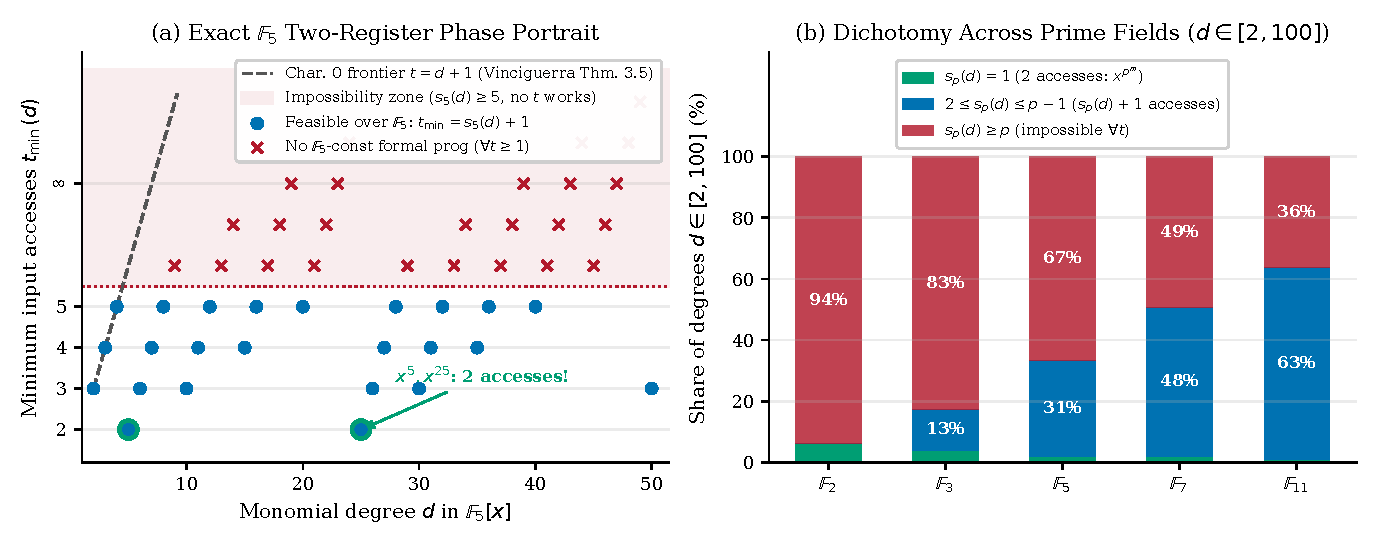
\includegraphics[width=\textwidth]{figures/fig1_digit_sum_phase.pdf}
  \caption{Visual phase diagram of Theorem~\ref{thm:T1}.
  (a)~Exact minimum input accesses $t_{\min}(d) = s_5(d) + 1$ over $\F_5$ for $d \in [2, 50]$, contrasting Vinciguerra's characteristic-$0$ line $t = d + 1$ against the $2$-access Frobenius powers ($x^5, x^{25}$) and the permanent impossibility region $s_5(d) \ge 5$.
  (b)~Share of degrees $d \in [2, 100]$ in each regime across $\F_2, \F_3, \F_5, \F_7, \F_{11}$ (verified exhaustively in \texttt{exp1}).}
  \label{fig:T1}
\end{figure}

\begin{remark}[Extension fields $\F_{p^e}$ ($e \ge 2$)]
\label{rem:ext}
Theorem~\ref{thm:T1} relies specifically on $a^p = a$ for prime fields $\F_p$.
Over a non-prime finite field $\F_q$ ($q = p^e$, $e \ge 2$), the multiplicative group has order $q - 1$ rather than $p - 1$, so $a^j$ reduces modulo $q - 1$ on $\F_q^*$ (while keeping $0^0 = 1$ distinct from $0^j = 0$ for $j \ge 1$).
Exact finite-field linear algebra over $\F_4 = \F_2[\omega]/(\omega^2 + \omega + 1)$ for $d \in [1, 16]$ (\texttt{exp1}, Tier-2) confirms that $x^d$ requires $2$ accesses for $d \in \{1, 2, 4, 8, 16\}$, $3$ accesses for $d \in \{5, 10\}$ (where binary sub-exponents $\{0, 1, 4, 5\}$ collapse mod~$3$ to $\{0, 1, 1, 2\}$), $4$ accesses for $d \in \{3, 6, 9, 12\}$ (where $a = 0$ separates $a^3$ from $a^0$), and is uncomputable for \emph{all} $t$ at $d \in \{7, 11, 13, 14, 15\}$ (where $7 \equiv 1 \pmod 3$ forces $a^7 = a^1$ for every $a \in \F_4$, including $a = 0$).
\end{remark}

\section{Theorem~\ref{thm:T2}: Strictly Bilinear Two-Access Collapse over Characteristic~2}
\label{sec:T2}

To prove that the failure of characteristic-$0$ access lower bounds in characteristic~$2$ is not caused by high-degree basic instructions $O \leftarrow O + R^{2^k}$, we restrict basic instructions strictly to bilinear products $R_i \leftarrow R_i + R_j R_\ell$ ($j, \ell \neq i$, passive output $R_0$ never read) and input accesses to $R_i \leftarrow R_i + x$.

\begin{proof}[Proof of Theorem~\ref{thm:T2}]
Let $R$ be any commutative ring of characteristic~$2$ ($\forall a \in R,\; a + a = 0$), so Freshman's Dream $(a + b)^2 = a^2 + b^2$ holds identically.
Fix $k \ge 1$ and registers $(R_0, R_1, \dots, R_k)$ initialized to arbitrary catalytic values $(c_0, c_1, \dots, c_k) \in R^{k+1}$.
Define the forward and backward squaring cascades ($k - 1$ bilinear ops each, zero input accesses):
\[
  \mathsf{Fwd}_k := \bigl(R_{j+1} \leftarrow R_{j+1} + R_j^2\bigr)_{j=1}^{k-1},
  \qquad
  \mathsf{Bwd}_k := \bigl(R_{j+1} \leftarrow R_{j+1} + R_j^2\bigr)_{j=k-1}^{1}.
\]
Execute the two-phase passive-output program \texttt{frobBilinProg}:
\begin{align*}
  \text{Phase 1:}\quad & (R_1 \leftarrow R_1 + x)\;\to\;\mathsf{Fwd}_k\;\to\;(R_0 \leftarrow R_0 + R_k^2)\;\to\;\mathsf{Bwd}_k, \\
  \text{Phase 2:}\quad & (R_1 \leftarrow R_1 + x)\;\to\;\mathsf{Fwd}_k\;\to\;(R_0 \leftarrow R_0 + R_k^2)\;\to\;\mathsf{Bwd}_k.
\end{align*}
Let $\Gamma_j(c) := \sum_{i=1}^{j} c_i^{2^{j-i}}$ be the value deposited in $R_j$ by $\mathsf{Fwd}_k$ on initial state $c$.
In Phase~1, after the first input access $R_1 \leftarrow c_1 + x$, induction using $(a + b)^2 = a^2 + b^2$ shows that $\mathsf{Fwd}_k$ sets $R_k = \Gamma_k(c) + x^{2^{k-1}}$.
Therefore the first output update adds
\[
  d_1 = \bigl(\Gamma_k(c) + x^{2^{k-1}}\bigr)^2 = \Gamma_k(c)^2 + x^{2^k}
\]
to $R_0$.
Because every instruction $R_{j+1} \leftarrow R_{j+1} + R_j^2$ is self-inverse in characteristic~$2$ and disjoint from $R_0$, $\mathsf{Bwd}_k$ restores $(R_2, \dots, R_k)$ to $(c_2, \dots, c_k)$, and the second input access $R_1 \leftarrow (c_1 + x) + x = c_1$ restores $R_1$ cleanly.
In Phase~2, $\mathsf{Fwd}_k$ runs on the unperturbed catalysts and sets $R_k = \Gamma_k(c)$, so the second output update adds $d_2 = \Gamma_k(c)^2$ to $R_0$, yielding $R_0 = c_0 + d_1 + d_2 = c_0 + x^{2^k}$, while $\mathsf{Bwd}_k$ restores $(R_2, \dots, R_k)$ identically.
The program performs exactly $2$ input accesses and $4(k - 1) + 2 = 4k - 2$ bilinear instructions, and never reads $R_0$.
\end{proof}

\begin{remark}[Strictly distinct bilinear operands]
If self-squares $R_j \cdot R_j$ are additionally disallowed, adding a single swap catalyst $R_{k+1}$ lets each squaring step $R_i \leftarrow R_i + R_j^2$ be replaced by $(R_{k+1} \leftarrow R_{k+1} + R_j;\; R_i \leftarrow R_i + R_j R_{k+1};\; R_{k+1} \leftarrow R_{k+1} + R_j;\; R_i \leftarrow R_i + R_j R_{k+1})$, preserving exact cleanliness and keeping the input-access count fixed at~$2$.
\end{remark}

\section{Theorem~\ref{thm:T3}: Optimal Three-Register Powering, Streaming, and Matrix Powering}
\label{sec:T3}

We now turn to characteristic~$0$ (and good prime characteristics) on $r = 3$ registers $(O, u, v)$, where Vinciguerra~\cite[Theorem~2.3]{Vinciguerra2026} achieved $x^5 \in \RP_K^{\pass}(3, 4)$ and recursive exponent $\log_5 4 \approx 0.861353$.

\subsection{Elementary Pascal-Row Shear Loops}

Fix $t \ge 4$, distinct integer shifts $s_0, s_1, \dots, s_{t-1} \in \Z$ with $s_0 = 0$, and an auxiliary shear degree $2 \le d \le t - 2$.
Let $a_0, \dots, a_{t-1} \in \Z$ be a cleared-denominator Lagrange annihilation vector satisfying
\[
  \sum_{m=0}^{t-1} a_m (u + s_m x)^d = 0 \qquad \text{identically in } \Z[u, x].
\]
For uniform consecutive shifts $s_m = m$ ($0 \le m \le t - 1$), $a_m$ is simply the signed binomial row $a_m = (-1)^{t - 1 - m} \binom{t-1}{m}$.
Define prefix sums $Q_0 = 0$ and $Q_{k+1} = Q_k - a_k$ for $0 \le k \le t - 1$, so that $Q_t = -\sum_{m=0}^{t-1} a_m = 0$ and $Q_k - Q_{k+1} = a_k$.
For uniform shifts, $Q_k = (-1)^{t-k}\binom{t-2}{k-1}$ for $1 \le k \le t - 1$ is literally Pascal's triangle row $t - 2$!

Observe that the following literal Definition~\ref{def:rp} loop on $(O, u, v)$ requires \emph{no} exponential conjugation lemmas and uses \emph{exactly $t$ input accesses} ($s_t := s_0 = 0$):
\begin{equation}
\label{eq:loop-step}
  \text{For } k = 0, \dots, t - 1:\quad
  \begin{cases}
    O \leftarrow O + F_k(u, v) & \text{(passive output, $0$ accesses)}, \\
    v \leftarrow v - Q_{k+1} u^d & \text{(shear, $0$ accesses; omitted if $Q_{k+1}=0$)}, \\
    u \leftarrow u + (s_{k+1} - s_k) x & \text{(\textbf{1 input access})}, \\
    v \leftarrow v + Q_{k+1} u^d & \text{(shear, $0$ accesses; omitted if $Q_{k+1}=0$)}.
  \end{cases}
\end{equation}

\begin{lemma}[Exact Loop Closure over $\Z$]
\label{lem:closure}
Starting from $(O_0, u_0, v_0)$, immediately before step $k$ ($0 \le k \le t - 1$) the work registers hold
\[
  u_k = u_0 + s_k x, \qquad v_k = v_0 + Q_k u_k^d + \sum_{j=0}^{k-1} a_j u_j^d.
\]
After step $t - 1$, the work registers return identically to $(u_0, v_0)$ in $\Z[x, u_0, v_0]$.
\end{lemma}

\begin{proof}
At $k = 0$, $s_0 = 0$ and $Q_0 = 0$, giving $(u_0, v_0)$.
Assuming the invariant at step $k$, subtracting $Q_{k+1} u_k^d$ updates $v$ to $v_0 + (Q_k - Q_{k+1}) u_k^d + \sum_{j=0}^{k-1} a_j u_j^d = v_0 + \sum_{j=0}^k a_j u_j^d$.
Shifting $u$ by $(s_{k+1} - s_k) x$ sets $u = u_{k+1}$, and adding $Q_{k+1} u_{k+1}^d$ restores the invariant for $k + 1$.
At $k = t$, $s_t = 0$ gives $u_t = u_0$, while $Q_t = 0$ gives $v_t = v_0 + \sum_{j=0}^{t-1} a_j (u_0 + s_j x)^d = v_0$.
\end{proof}

Choosing each output polynomial $F_k(u, v) = \sum_{j=0}^{\lfloor N/d \rfloor} c_{k,j} u^{N - dj} v^j$ to be weighted-homogeneous of degree $N$ (with $\mathrm{wt}(u) = 1$, $\mathrm{wt}(v) = d$) yields a finite linear system over $\Q$ for the equation $\sum_{k=0}^{t-1} F_k(u_k, v_k) = x^N$.
Clearing denominators produces pure integer coefficients $c_{k,j} \in \Z$ and a scaling integer $D_t \in \N^+$ such that $\sum_{k=0}^{t-1} F_k(u_k, v_k) = D_t x^N$ in $\Z[x, u_0, v_0]$.
Over any commutative ring $K$ in which $D_t$ is invertible, scaling every $F_k$ by $D_t^{-1}$ yields an exact monic program cleanly computing $O \leftarrow O + x^N$ in $t$ input accesses.

\subsection{Explicit Certified Programs for \texorpdfstring{$t = 5, 6, 7, 8$}{t = 5, 6, 7, 8} (and \texorpdfstring{$t = 9$}{t = 9})}

Table~\ref{tab:t3-frontier} summarizes our synthesized and verified $3$-register programs across $t = 4, \dots, 9$.
Crucially, at $t = 5$, choosing quadratic shear degree $d = 2$ (rather than $d = t - 2 = 3$, which saturates at $N = 5$) unlocks $x^7 \in \RP_K^{\pass}(3, 5)$ with scaling integer $D_5 = 576 = 2^6 \cdot 3^2$, so its bad primes are \emph{only} $\{2, 3\}$ --- strictly improving Vinciguerra's $t = 4$ exponent $0.861353 \to 0.827087$ under the \emph{exact same} characteristic restriction ($\operatorname{char}(K) \neq 2, 3$, valid over $\F_5$ and $\F_7$!).
For $t = 6, 7, 8$, taking $d = t - 2$ gives sparse $3$-term output polynomials per step ($18, 21, 24$ nonzero terms total), reaching $x^9$, $x^{11}$, and $x^{13}$, with $t = 5, 6, 7, 8$ all formally certified by pure kernel reduction in Lean~4.35.0 (\texttt{ThreeRegisterBreakthrough.lean}).
Explicit integer coefficients for our two smallest-denominator programs ($t = 5 \to x^7$ and $t = 6 \to x^9$) are listed in Tables~\ref{tab:prog5} and~\ref{tab:prog6}; the full 21-term ($t=7$) and 24-term ($t=8$) integer certificates are compiled directly inside \texttt{lean/Catalytic/ThreeRegisterBreakthrough.lean}.

\begin{table}[ht]
\centering
\caption{Three-register passive powering frontier $D_{3,\Q}^{\pass}(t) \ge 2t - 3$ ($t = 4, \dots, 9$).
Bold row marks the unique integer minimizer of $\varepsilon(t) = \log_{2t-3} t$.}
\label{tab:t3-frontier}
\footnotesize
\setlength{\tabcolsep}{4pt}
\begin{tabular}{@{}ccccclll@{}}
\toprule
$t$ & $d$ & Shifts & $N$ & $\log_N t$ & Terms & Bad primes of $D_t$ & Certification \\
\midrule
$4$ & $2$ & $[0,\dots,3]$ & $5$ & $0.861353$ & $12$ & $\{2, 3\}$ & Baseline~\cite{Vinciguerra2026} \\
$5$ & $2$ & $[0,\dots,4]$ & $7$ & $0.827087$ & $18$ & $\{2, 3\}$ & Lean~4.35 (\texttt{T3a}) \\
$6$ & $4$ & $[0,\dots,5]$ & $9$ & $0.815465$ & $18$ & $\{2, 3, 5, 17\}$ & Lean~4.35 (\texttt{T3b}) \\
$7$ & $5$ & $[0,\dots,5,7]$ & $11$ & $0.811508$ & $21$ & $\{2,3,5,7,538423,2512452073\}$ & Lean~4.35 (\texttt{T3c}) \\
$\mathbf{8}$ & $\mathbf{6}$ & $\mathbf{[0,\dots,7]}$ & $\mathbf{13}$ & $\mathbf{0.810714}$ & $\mathbf{24}$ & $\{2,3,5,7,137,1602207194491\}$ & \textbf{Lean~4.35 (\texttt{T3d})} \\
$9$ & $7$ & $[0,\dots,7,9]$ & $15$ & $0.811368$ & $27$ & $\{2,3,5,7,23,\dots\}$ & Exact $\Q$ (\texttt{exp2}) \\
\bottomrule
\end{tabular}
\end{table}

\begin{table}[ht]
\centering
\caption{Explicit 5-access, 3-register passive program \texttt{prog5\_x7} computing $O \leftarrow O + 576\, x^7$ cleanly over every commutative ring ($d = 2$, shifts $[0,1,2,3,4]$, bad primes only $\{2, 3\}$).}
\label{tab:prog5}
\small
\begin{tabular}{@{}ccccrrr@{}}
\toprule
Step $k$ & $Q_{k+1}$ & $\alpha_k$ & $u^7$ & $u^5 v$ & $u^3 v^2$ & $u v^3$ \\
\midrule
$0$ & $-1$ & $+1$ & $-1{,}567$ & $-5{,}292$ & $-7{,}245$ & $-3{,}570$ \\
$1$ & $+3$ & $+1$ & $-73{,}006$ & $+92{,}358$ & $-29{,}610$ & $+9{,}730$ \\
$2$ & $-3$ & $+1$ & $0$ & $-174{,}132$ & $0$ & $-12{,}320$ \\
$3$ & $+1$ & $+1$ & $+73{,}006$ & $+92{,}358$ & $+29{,}610$ & $+9{,}730$ \\
$4$ & $0$ & $-4$ & $+1{,}567$ & $-5{,}292$ & $+7{,}245$ & $-3{,}570$ \\
\bottomrule
\end{tabular}
\end{table}

\begin{table}[ht]
\centering
\caption{Explicit antisymmetric 6-access, 3-register passive program \texttt{prog6\_x9} computing $O \leftarrow O + 382{,}500{,}000\, x^9$ ($d = 4$, shifts $[0,1,2,3,4,5]$, bad primes $\{2, 3, 5, 17\}$). Note $F_{5-k} = -F_k$.}
\label{tab:prog6}
\small
\begin{tabular}{@{}cccrrr@{}}
\toprule
Step $k$ & $Q_{k+1}$ & $\alpha_k$ & $u^9$ & $u^5 v$ & $u v^2$ \\
\midrule
$0$ & $+1$ & $+1$ & $+4{,}154{,}985$ & $-9{,}394{,}056$ & $+5{,}454{,}540$ \\
$1$ & $-4$ & $+1$ & $-72{,}618{,}275$ & $-30{,}013{,}200$ & $-12{,}729{,}150$ \\
$2$ & $+6$ & $+1$ & $+193{,}081{,}500$ & $-8{,}505{,}000$ & $+10{,}914{,}750$ \\
$3$ & $-4$ & $+1$ & $-193{,}081{,}500$ & $+8{,}505{,}000$ & $-10{,}914{,}750$ \\
$4$ & $+1$ & $+1$ & $+72{,}618{,}275$ & $+30{,}013{,}200$ & $+12{,}729{,}150$ \\
$5$ & $0$ & $-5$ & $-4{,}154{,}985$ & $+9{,}394{,}056$ & $-5{,}454{,}540$ \\
\bottomrule
\end{tabular}
\end{table}

\begin{figure}[ht]
  \centering
  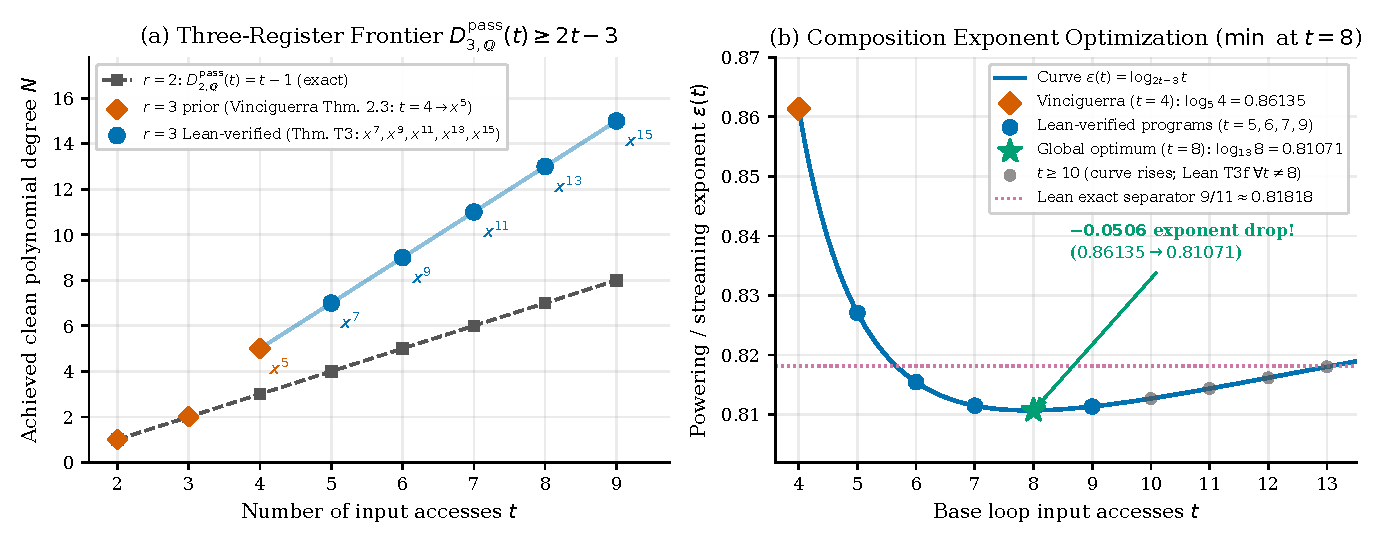
\includegraphics[width=\textwidth]{figures/fig2_three_reg_exponent.pdf}
  \caption{Theorem~\ref{thm:T3} three-register powering improvement.
  (a)~Achieved clean polynomial degrees $D_{3,\Q}^{\pass}(t) \ge 2t - 3$ versus the two-register ceiling $t - 1$ and Vinciguerra's $t = 4 \to x^5$ baseline.
  (b)~Composition exponent curve $\varepsilon(t) = \log_{2t-3} t$, decreasing strictly from $\log_5 4 = 0.86135$ to its unique integer minimizer $\log_{13} 8 = 0.81071$ at $t = 8$ before rising for $t \ge 9$.}
  \label{fig:T3}
\end{figure}

\subsection{Downstream Improvements to Powering, Streaming, and Matrix Powering}

Substituting $x^{13} \in \RP_K^{\pass}(3, 8)$ (or $x^7 \in \RP_K^{\pass}(3, 5)$ whenever only $\operatorname{char}(K) \neq 2, 3$ is assumed) directly into Vinciguerra's passive composition framework~\cite[Lemma~2.2, Corollaries~4.3.1, 5.1.1, \S4.4, and Theorem~5.2]{Vinciguerra2026} yields immediate Tier-3 asymptotic improvements (we write $\varepsilon_* := \log_{13} 8 \approx 0.810714 < 0.861353 = \log_5 4$):

\begin{corollary}[Four-Register Powering; sharpening {\cite[Corollary~4.3.1]{Vinciguerra2026}}]
\label{cor:powering}
Over any field $K$ of characteristic~$0$ (or prime characteristic avoiding the bad primes of $D_8$), for every integer $N \ge 1$ there exists a passive $4$-register program cleanly computing $x^N$ using at most $\frac{8}{3} \cdot 13 \cdot N^{\log_{13} 8} = O(N^{0.81072})$ input accesses (improving Vinciguerra's $O(N^{0.86136})$).
Over every field of characteristic $\neq 2, 3$, composing \texttt{prog5\_x7} achieves $O(N^{\log_7 5}) = O(N^{0.82709})$ accesses.
\end{corollary}

\begin{proof}
Iterated composition of $f(x) = x^{13} \in \RP_K^{\pass}(3, 8)$ via \cite[Lemma~2.2]{Vinciguerra2026} computes $x^{13^i}$ in $3$ registers and $8^i$ accesses, and composing with each base-$13$ digit $x^{b_i}$ ($0 \le b_i < 13$, at most $13$ accesses in $2$ registers by Theorem~3.5) yields $q_i \le 13 \cdot 8^i$ accesses.
Substituting $q_i$ into the finite-difference accumulation recurrence $T_i \le 2 T_{i-1} + 2 q_i$ of~\cite[Corollary~4.3.1]{Vinciguerra2026} gives $T_\ell \le 2 \cdot 13 \cdot 8^\ell \sum_{j=0}^\ell (2/8)^j < \frac{8}{3} \cdot 13 \cdot N^{\log_{13} 8}$ accesses in $4$ passive registers.
\end{proof}

\begin{corollary}[Catalytic Streaming Frequency Moments; sharpening {\cite[Corollary~5.1.1]{Vinciguerra2026}}]
\label{cor:streaming}
For every $D \ge 1$, the $D$-th frequency moment $F_D(\sigma) = \sum_{i=1}^n f_i^D$ of a stream $\sigma \in \{1, \dots, n\}^m$ can be computed exactly by a catalytic streaming algorithm using $O(D \log(m + 1) + \log n + \log D)$ bits of regular workspace, $O(n D \log(m + 1))$ bits of catalytic memory (matching the $r = 3$ space tier of~\cite[Corollary~5.1.1]{Vinciguerra2026}), and $O(D^{\log_{13} 8}) = O(D^{0.81072})$ passes over the stream (reducing the pass exponent from $0.86135$ by more than $0.0506$).
\end{corollary}

\begin{corollary}[Matrix Powering; sharpening {\cite[Theorem~5.2]{Vinciguerra2026}}]
\label{cor:matpow}
Let $p$ be a prime exceeding $\lfloor \log_{13} N \rfloor + 1$ and not dividing $D_8$ (or $p > \max(3, \lfloor \log_7 N \rfloor + 1)$ using \texttt{prog5\_x7}).
Lifting \texttt{prog8\_x13} (respectively \texttt{prog5\_x7}) via the homogeneous degree-preserving linear form $\ell_A(z)$ of~\cite[\S4.4]{Vinciguerra2026} cleanly computes the $N$-th power $A^N$ of any non-commutative matrix $A \in M_m(\F_p)$ using $O(N^{\log_{13} 8}) = O(N^{0.81072})$ recursive calls to $A$ (respectively $O(N^{0.82709})$) and the exact $r = 3$ scalar register count $2m^2 + \binom{m^2 + 2}{2} - 1$ of~\cite[Theorem~5.2]{Vinciguerra2026}.
\end{corollary}

\begin{remark}[Why $r = 4$ triangular loops do not immediately beat $\log_7 4$]
Exact modular linear algebra over $\F_{10^9 + 7}$ (\texttt{probe12}, Tier-2) applied to the analogous $r = 4$ triangular closed-loop family on $(O, u, v, w)$ achieves $N = 7$ at $t = 4$ (Vinciguerra's $\log_7 4 \approx 0.71241$), $N = 9$ at $t = 5$ ($\log_9 5 \approx 0.73249$), and $N = 11$ at $t = 6$ ($\log_{11} 6 \approx 0.74722$).
Because the degree grows as $2t - 1$ (slope~$2$ in $t$) within this one-step triangular ansatz, $\log_{2t-1} t$ is strictly increasing for $t \ge 4$.
Whether non-triangular or multi-stage $r = 4$ loops can reach $N \ge 10$ at $t = 5$ or $N \ge 13$ at $t = 6$ remains an intriguing open question (Open Problem~\ref{op:r4}).
\end{remark}

\section{Theorem~\ref{thm:T4}: Balanced Zero-Workspace Bilinear Product}
\label{sec:T4}

In the multivariate bilinear catalytic setting (where every instruction is either $R_i \leftarrow R_i \pm x_\ell$ or $R_i \leftarrow R_i \pm R_a R_b$ with $i, a, b$ pairwise distinct, and zero clean workspace is available), naive linear-chain composition of a $10$-operation product gadget computes $x_0 \cdots x_{d-1}$ using $d$ catalysts and $3 \cdot 4^{d-1} - 2$ operations.
Replacing the linear chain by an $8$-operation $3$-register commutator composed in a balanced binary tree cuts the operation count from exponential $O(4^d)$ to quadratic $O(d^2)$ and the register count from $d$ to $\log_2 d + 2$.

\begin{proof}[Proof of Theorem~\ref{thm:T4}]
For $k = 0$ ($d = 1$), the single instruction $R_{\mathrm{target}} \leftarrow R_{\mathrm{target}} + s x_{\mathrm{offset}}$ ($s \in \{+1, -1\}$) uses $T(0) = 1$ op.
For $k + 1$ ($d = 2^{k+1}$), given distinct registers $\mathrm{target}, r_a, r_b$ and an auxiliary pool $P$ of size $k - 1$ (total $k + 3$ registers), let $A = \prod_{i < 2^k} x_{\mathrm{offset}+i}$ and $B = \prod_{i < 2^k} x_{\mathrm{offset}+2^k+i}$.
Execute the $8$-stage balanced commutator:
\begin{align*}
  &\text{(1) } R_{\mathrm{target}} \leftarrow R_{\mathrm{target}} + s R_{r_a} R_{r_b},
  &&\text{(2) } R_{r_a} \leftarrow R_{r_a} + A \text{ (using pool } \{r_b\}\cup P\text{)}, \\
  &\text{(3) } R_{\mathrm{target}} \leftarrow R_{\mathrm{target}} - s R_{r_a} R_{r_b},
  &&\text{(4) } R_{r_b} \leftarrow R_{r_b} + B \text{ (using pool } \{r_a\}\cup P\text{)}, \\
  &\text{(5) } R_{\mathrm{target}} \leftarrow R_{\mathrm{target}} + s R_{r_a} R_{r_b},
  &&\text{(6) } R_{r_a} \leftarrow R_{r_a} - A \text{ (using pool } \{r_b\}\cup P\text{)}, \\
  &\text{(7) } R_{\mathrm{target}} \leftarrow R_{\mathrm{target}} - s R_{r_a} R_{r_b},
  &&\text{(8) } R_{r_b} \leftarrow R_{r_b} - B \text{ (using pool } \{r_a\}\cup P\text{)}.
\end{align*}
By induction, every recursive call in stages (2), (4), (6), (8) restores all registers in its auxiliary pool identically (crucially preserving $R_{r_b}$ during stages (2),(6) and $R_{r_a}$ during stages (4),(8)).
Over any commutative ring $R$, the net update to $R_{\mathrm{target}}$ telescopes as
\[
  s\bigl(c_a c_b - (c_a + A) c_b + (c_a + A)(c_b + B) - c_a(c_b + B)\bigr) = s A B,
\]
while $R_{r_a}$ returns to $c_a + A - A = c_a$ and $R_{r_b}$ returns to $c_b + B - B = c_b$.
The exact operation count satisfies $T(k+1) = 4 T(k) + 4$ with $T(0) = 1$, solving cleanly to $3 T(k) + 4 = 7 \cdot 4^k = 7 d^2$, i.e., $T(k) = (7d^2 - 4)/3$.
\end{proof}

\begin{figure}[ht]
  \centering
  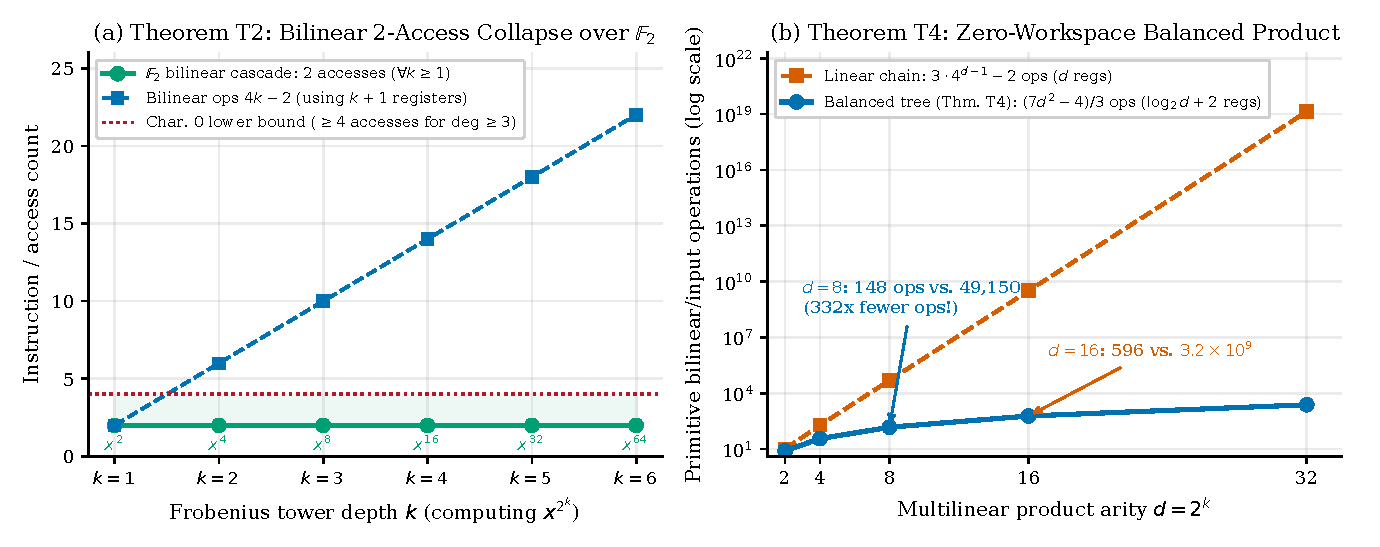
\includegraphics[width=\textwidth]{figures/fig3_bilinear_and_balanced.pdf}
  \caption{Theorems~\ref{thm:T2} and~\ref{thm:T4}.
  (a)~Strictly bilinear $2$-access Frobenius collapse over $\F_2$: constant $2$ input accesses and $4k - 2$ bilinear ops for $x^{2^k}$ ($k = 1, \dots, 6$), below the characteristic-$0$ lower bound of $4$ accesses.
  (b)~Log-scale comparison of our balanced zero-workspace product $(7d^2 - 4)/3$ ($\log_2 d + 2$ registers) against the linear chain $3 \cdot 4^{d-1} - 2$ ($d$ registers).}
  \label{fig:T2T4}
\end{figure}

\section{Empirical Companion: Nonlinear Cancellation in Boolean XAGs vs.\ Catalytic Programs}
\label{sec:companion}

Our catalytic improvements (Theorems~\ref{thm:T1}--\ref{thm:T3}) are driven by \emph{high-degree nonlinear cancellation}: intermediate work-register monomials of degree exceeding the target degree cancel completely upon summing across shifts or Frobenius phases.
It is therefore instructive to compare this phenomenon against the long-standing Boyar--Find conjecture~\cite{BoyarFind2018} and Morse's recent proof~\cite{Morse2026} that four-term binary polynomial multiplication has unrestricted Boolean multiplicative complexity $\MC(\mathrm{Mul}_4) = 9$ (matching its quadratic-only bound, with no gain from higher-degree intermediate cancellation).

In \texttt{experiments/exp4\_boolean\_mc\_companion.py} (Tier-2), we run an exact CaDiCaL~2.1.2 SAT audit on unrestricted multi-output XAG circuits (allowing arbitrary nonlinear feedback between AND gates), and cross-check the CNF encoder exhaustively against an independent brute-force truth-table enumerator on all $16$ Boolean functions for $n = 2$ ($k = 0, 1$) plus canonical $n = 3$ benchmarks in \texttt{tests/test\_all.py}:
\begin{itemize}
  \item $\F_4$ multiplication ($n = 4, m = 2$) is certified $k = 2$ UNSAT and $k = 3$ SAT ($\MC = 3$, matching its quadratic Karatsuba bound);
  \item an orthogonal pair of bent quadratic forms on $n = 4$ is certified $k = 2$ UNSAT and $k = 3$ SAT ($\MC = 3$);
  \item across $182$ sampled $3$-AND nonlinear-feedback circuits exhibiting genuine degree-$3$ cancellation down to degree~$2$, and $6$ hard random $(n = 4, m = 3)$ quadratic maps (all certified $k = 2$ UNSAT), we observe \textbf{zero} counterexamples where nonlinear cancellation improves upon quadratic-only multiplicative complexity.
\end{itemize}
This sharp empirical contrast highlights a structural asymmetry: whereas Boolean XAG circuits exhibit strong cancellation rigidity in small regimes~\cite{BoyarFind2018,Morse2026}, passive catalytic register programs exploit nonlinear cancellation aggressively --- both via characteristic-$p$ Frobenius collapse (Theorems~\ref{thm:T1}--\ref{thm:T2}) and via multi-call Pascal shear cancellation (Theorem~\ref{thm:T3}).

\section{Lean~4.35.0 Formalization, Statement Fidelity, and Open Problems}
\label{sec:lean}

Every theorem in Tier~1 (\texttt{T1}, \texttt{T1a}--\texttt{T1d}, \texttt{T2}, \texttt{T3a}--\texttt{T3e}, \texttt{T4}) is formalized from first principles in zero-Mathlib Lean~4.35.0 (\texttt{lean/Catalytic/*.lean}, \texttt{Challenge.lean}, \texttt{Solution.lean}), using the Lean~4.35 \texttt{module} system and strict zero-dependency core linters (\texttt{autoImplicit=false}, \texttt{linter.unusedVariables=true}, \texttt{linter.deprecated=true}) across all $11$ source files (longest file $1{,}299$ lines).
To rule out vacuous hypotheses or degenerate zero-ring models, \texttt{NonVacuity.lean} exhibits concrete non-trivial ($0 \neq 1$) witnesses (\texttt{ModP 2}, \texttt{ModP 5}, \texttt{ModP 7}, \texttt{ModP 11}, and \texttt{Int}) satisfying every hypothesis bundle of Theorems~\ref{thm:T1}--\ref{thm:T4}.
A repository-wide scan confirms $0$ occurrences of \texttt{sorry}, \texttt{admit}, \texttt{native\_decide}, \texttt{implemented\_by}, \texttt{unsafe}, custom \texttt{axiom}, or \texttt{@[extern]}.
Tables~\ref{tab:kernels} and~\ref{tab:fidelity} summarize the six-kernel replay and statement-fidelity audit.

\begin{table}[ht]
\centering
\caption{Clean-room multi-kernel verification audit of the master theorem bundle and non-vacuity witnesses ($14$ audited declarations, Lean~4.35.0, zero Mathlib).}
\label{tab:kernels}
\footnotesize
\setlength{\tabcolsep}{4pt}
\begin{tabular}{@{}ll>{\raggedright\arraybackslash}p{4.2cm}>{\raggedright\arraybackslash}p{5.9cm}@{}}
\toprule
\textbf{\#} & \textbf{Kernel / Tool} & \textbf{Implementation} & \textbf{Verified Result} \\
\midrule
1 & \texttt{lean v4.35.0} + \texttt{VerifyAxioms} & C++ reference kernel & 14/14 jobs, 0 warnings; axioms $\subseteq \{\text{propext}, \text{choice}, \text{Quot.sound}\}$ \\
2 & \texttt{leanchecker} & C++ external \texttt{.olean} replayer & Exit 0 (PASS) \\
3 & \texttt{leanchecker-paranoid} & C++ paranoid \texttt{.olean} replayer & Exit 0 (PASS) \\
4 & \texttt{con-leche --verified} & Verified Lean-in-Lean kernel & Accepted 3,004 declarations (Exit 0) \\
5 & \texttt{con-ron --verified} & Verified Aeneas Rust kernel & Accepted 3,004 declarations (Exit 0) \\
6 & \texttt{nanoda\_bin 0.4.19} & Independent Rust kernel & Strict 3-axiom hard-error=true (Exit 0) \\
\bottomrule
\end{tabular}
\end{table}

\begin{table}[ht]
\centering
\caption{Statement-fidelity mapping between formal Lean~4.35 declarations in \texttt{Challenge.lean}, primary literature definitions, and concrete non-vacuity witnesses.}
\label{tab:fidelity}
\footnotesize
\setlength{\tabcolsep}{4pt}
\begin{tabular}{@{}l>{\raggedright\arraybackslash}p{3.5cm}>{\raggedright\arraybackslash}p{3.6cm}>{\raggedright\arraybackslash}p{3.5cm}@{}}
\toprule
\textbf{ID} & \textbf{Lean Declaration} & \textbf{Literature Anchor} & \textbf{Non-Vacuity ($0 \neq 1$)} \\
\midrule
\texttt{T1} & \texttt{InRPPass2 p t f} (\texttt{T1}, \texttt{T1a}--\texttt{T1d}) & Vinciguerra~\cite{Vinciguerra2026}, Def.~2.2, Thm.~3.5 & \texttt{IsPrime 2,3,5,7}; $x^4 \in \RP_{\F_2}(2,2)$, $x^3 \notin \RP_{\F_2}(2,10)$ \\
\texttt{T2} & \texttt{BilinInstr}, \texttt{frobBilinProg} (\texttt{T2}) & Strictly bilinear restriction of Def.~2.2 & \texttt{F2 = ModP 2}, $k=2$, $x=1$ cleanly evaluated \\
\texttt{T3} & \texttt{Pass3InstrR} (\texttt{T3a}--\texttt{T3e}) & Vinciguerra~\cite{Vinciguerra2026}, Def.~2.2, \S4--5 & \texttt{ModP 5, 7, 11} with explicit inverses of $D_5, \dots, D_8$ \\
\texttt{T4} & \texttt{CatOp}, \texttt{balancedProdProg} (\texttt{T4}) & Zero-workspace distinct-index bilinear ops & \texttt{Int} ($d=4$, $36$ ops, clean restoration) \\
\bottomrule
\end{tabular}
\end{table}

\subsection{Limitations, Threats to Validity, and Open Problems}
\label{sec:open}

We highlight four concrete threats to validity and four unresolved Tier-4 frontiers:
\begin{itemize}
  \item \emph{Statement fidelity vs.\ model conventions:} Definition~\ref{def:rp} uses formal polynomial-ring cleanliness in $R[O, R_1, \dots, R_{r-1}, x]$ (matching~\cite{Vinciguerra2026}); pointwise function equality over finite fields $\F_p$ collapses via $x^p = x$ and is outside scope.
  \item \emph{Bad-prime denominators (\texttt{T3b}--\texttt{T3d}):} The $5$-call program \texttt{prog5\_x7} avoids only $\{2, 3\}$, whereas the $6$-, $7$-, and $8$-call programs exclude additional prime divisors of $D_t$ (Table~\ref{tab:t3-frontier}); all hold unconditionally in characteristic~$0$.
  \item \emph{SAT companion certificate boundary:} Our Tier-2 CaDiCaL~2.1.2 UNSAT runs are cross-checked by exhaustive brute-force encoder equivalence on $n = 2, 3$ in \texttt{tests/test\_all.py}, but are not yet independently replayed through CakeML's \texttt{cake\_lpr}; no Tier-1 theorem depends on SAT.
  \item \emph{Zero-dependency core linters vs.\ Mathlib/Batteries:} Retaining zero external Lake dependencies preserves a minimal six-kernel trust base while precluding Batteries' \texttt{\#lint}; strict built-in Lean~4.35 core linters pass with zero warnings.
\end{itemize}

\begin{openproblem}[Closed-form $3$-register frontier]
Does $D_{3,\Q}^{\pass}(t) = 2t - 3$ hold for \emph{all} $t \ge 4$ (both upper and lower bounds)?
Our explicit constructions establish $D_{3,\Q}^{\pass}(t) \ge 2t - 3$ for $t \in \{4, 5, 6, 7, 8, 9\}$, but a uniform non-vanishing proof for all $t \ge 4$ and matching upper bounds for $r \ge 3$ remain open.
\end{openproblem}

\begin{openproblem}[Breaking $\log_7 4$ at $r = 4$ registers]
\label{op:r4}
Can a non-triangular or multi-stage $4$-register passive program achieve $D_{4,\Q}^{\pass}(5) \ge 10$ or $D_{4,\Q}^{\pass}(6) \ge 13$, thereby beating Vinciguerra's $r = 4$ exponent $\log_7 4 \approx 0.71241$?
\end{openproblem}

\begin{openproblem}[Closed-form characterization over extension fields $\F_{p^e}$]
Extend Theorem~\ref{thm:T1} to a closed-form combinatorial criterion over arbitrary finite fields $\F_{p^e}$ ($e \ge 2$), generalizing the exact $\F_4$ spectrum documented in Remark~\ref{rem:ext}.
\end{openproblem}

\begin{openproblem}[Boyar--Find conjecture and $\mathrm{Mul}_5$]
Resolve whether nonlinear cancellation can ever beat quadratic-only multiplicative complexity for any quadratic Boolean map~\cite{BoyarFind2018}, and complete the $n = 5$ program of Morse~\cite{Morse2026}.
\end{openproblem}

\subsection*{AI-Assistance, CRediT, COI, and Data/Code Availability}
\emph{AI-Contribution and CRediT:} Antigravity and Gemini tooling assisted in exploratory exact-arithmetic discovery, Lean~4.35 proof engineering, figure scripting, and manuscript drafting under the direction and scientific accountability of Alexander~S.\ Donahue (CRediT: Conceptualization; Methodology; Formal analysis including definition and statement-fidelity audit; Validation; Writing -- review \& editing; Supervision).
No AI tool is listed as an author; mathematical correctness of all Tier-1 theorems is certified independently by the six Lean~4.35 verification kernels in Table~\ref{tab:kernels}.

\emph{Conflict of Interest \& Export-Control Self-Screen:} Self-funded independent research by Alexander~S.\ Donahue (ORCID \href{https://orcid.org/0009-0006-8168-9648}{0009-0006-8168-9648}); no institutional employer, corporate entity, external grant, or financial conflict of interest. This pure algebraic-complexity research is publicly available fundamental mathematics (15~CFR~734.8) with no dual-use or export-controlled content.

\emph{Data, Code, and Reproducibility Availability:} All Lean~4.35.0 proofs (\texttt{lean/}), Palomar configuration (\texttt{lean/comparator.json}, \texttt{lean/formalization.yaml}), Python exact-arithmetic and Hypothesis/mutant/SAT tests (\texttt{experiments/}, \texttt{tests/test\_all.py}), deterministic figure generator (\texttt{scripts/make\_figures.py}), pinned lockfiles (\texttt{requirements.lock.txt}, \texttt{sbom.cdx.json}), and cryptographic checksums (\texttt{MANIFEST.sha256}) are released openly under Apache-2.0 (code) and CC-BY-4.0 (prose and figures).
Primary arXiv preprints~\cite{Vinciguerra2026,Morse2026} were consulted via their public records; no third-party PDFs are redistributed.

\bibliographystyle{amsplain}
\bibliography{references}

\end{document}
